\documentclass[main.tex]{subfiles} 
\begin{document}
\newpage
\section{Dive into Fuzzy Query-Answering Web Interface}
\label{sec:FuzzyQA}
\begin{figure}[htb]
\begin{center}
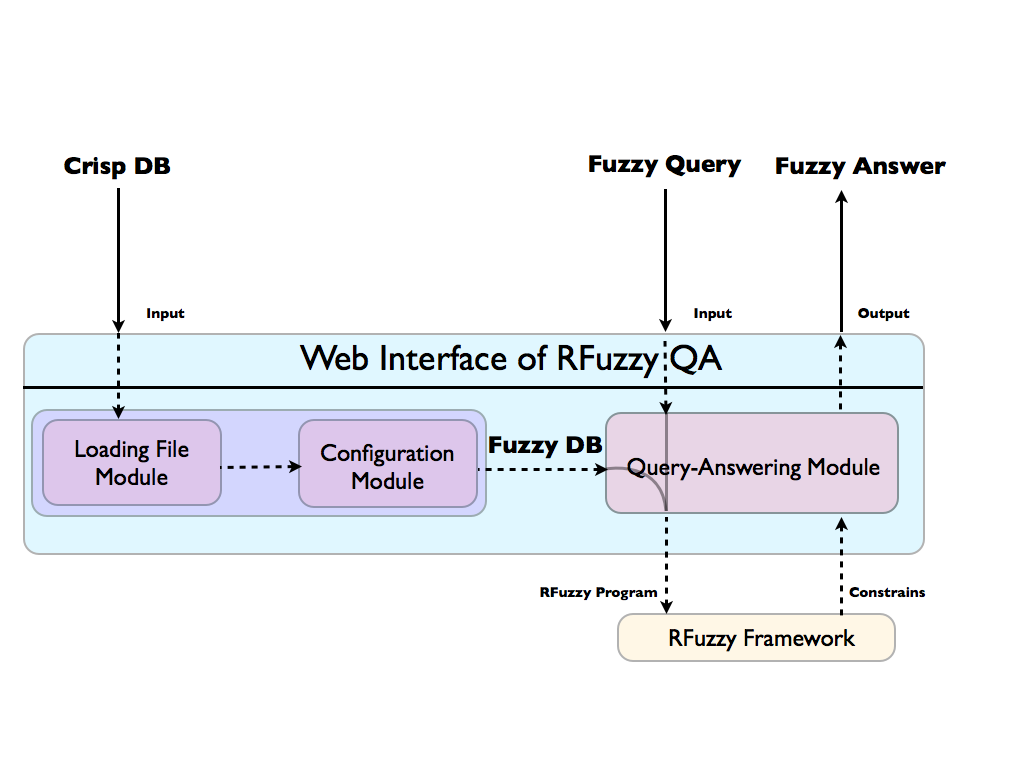
\includegraphics[scale=0.4]{FQAS.png}
\end{center}
\caption{Fuzzy Query-Answering System}
\label{fig:FQAS}
\end{figure}

%Introduction of FQAS
The framework of Fuzzy Query-Answering System (FQAS) is given in figure \ref{fig:FQAS}. FQAS receive crisp database and fuzzy query as input, and output fuzzy answer, which means users can ask fuzzy queries over crisp database. In FQAS, \textit{Loading File Module} (LFM) accepts crisp database, which parse the schema of database; \textit{Configuration Module} (CM) offers users to create fuzzy concepts over crisp database, as well as negation and quantification. Simply speaking, it generates a virtual fuzzy database upon crisp database; \textit{Query-Answering Module} (QAM) takes virtual fuzzy database and fuzzy query as input and generates a RFuzzy prolog program, which is passed to RFuzzy Framework to do the reasoning, QAM parses the result from RFuzzy Framework as fuzzy answer of FAQS.

In this section, the main three modules are presented in detail in section \ref{sec:LoadingFileModule}, \ref{sec:ConfigurationModule} and \ref{sec:QAModule}, respectively.
\subsection{Loading File Module}
\label{sec:LoadingFileModule}
Loading File Module offers users to choose a crisp database and its schema from local file system.
It parses database schema and generates  a table called Attribute to store information (name of attribute, type of attribute, range of attribute), on which fuzzy concepts are built.

\subsubsection{Database and its schema}
Crisp database is in a prolog file with extension ``.pl", and its schema is in a XML file with extension ``.xml". Crisp database is simply one predicate prolog program, the predicate is the name of table, and its arguments are terms of atom. Each atom is considered as an entry in the table. The schema of database is presented in .xml file, which stores table name, primary key and attributes information.
There are examples of crisp database in .pl file and its schema in .xml file.

%Explain db file
\begin{ex}
In .pl file, house is the only predicate, and it is the name of table. All the atoms in .pl file are entries of the table house.
\lstinputlisting{house.pl}
\end{ex}

%Explain db Schema file
\begin{ex}
As shown in .xml file, the name of table is house, the primary key is house\_code. The attributes of table house are type, size, number of rooms, price, distance from center, close to beach. The information about domain of each attribute is also included.
\lstinputlisting{house.xml}
\end{ex}

\subsubsection{How to use interface of Loading File Module}
The web interface of Loading File Module is shown in figure \ref{fig:LFI}. Three steps  to load a database.
\begin{enumerate}
\item Choose crisp database from Db selection box
\item Choose corresponding database schema from Xml selection box
\item Click Button Load
\end{enumerate}
In the last step, system stores file information in model ``InputFile" and parses .xml file into two models, one is ``Table", the other is ``Attribute". All the models are in file models.py.
\begin{figure}[htb]
\begin{center}
\leavevmode
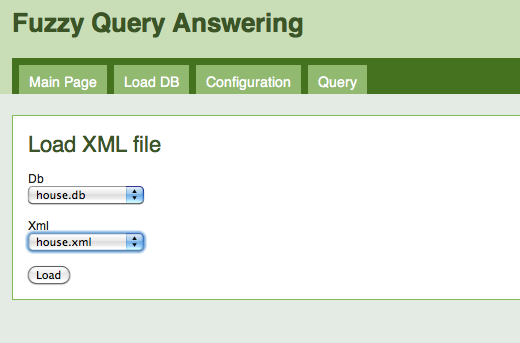
\includegraphics[scale=0.7]{LoadFile.png}
\end{center}
\caption{Loading File Interface}
\label{fig:LFI}
\end{figure}





\subsection{Configuration Module}
\label{sec:ConfigurationModule}

Configuration Module functions the configuration of fuzzy concepts over crisp database, negation and quantification of natural language. The crisp database is the one load it in the Loading File Module. Users are entitled to create and edit fuzzy concepts such as ``beautiful", ``old" by defining fuzzy functions over attributes in crisp database. Negations and quantifications can be created by defining the their functions over unit interval $[0,1]$.

\subsubsection{Fuzzy Concept}
Fuzzy concept is created over one of attributes in crisp database. For example, we can create fuzzy concept ``expensive" over attribute ``price". In this section, we formalize definition of fuzzy concept.
\begin{defin} \textbf{Fuzzy Concept}
Let $\mathcal{A}$ be a set of attributes, and $\mathcal{D}$ be a set of domain, that is $\mathcal{D}=\{(type, range) \mid type =\{Continuous, Discrete\}\}$. $g_{AD}$ is a function mapping  from attributes to domains, that is, $\mathcal{A} \rightarrow \mathcal{D}$. Suppose there existes fuzzy function $f_{D}$ is $\mathcal{D} \rightarrow [0,1]$. 

A fuzzy concept $FC$ is defined as a function $f_{FC}: \mathcal{A} \rightarrow [0,1]$. Indeed, $f_{FC}(att)= f_{D}(g_{AD}({att}))$, where $att \in \mathcal{A}$.
\end{defin}
\begin{ex} \textbf{Create fuzzy concept ``big"}
\label{ex:CreateFuzzyConcept}
As shown in house.xml, there exists an attribute ``size"  with its type ``Continuous (C)" and its range ``[(0,2500]]", which means an interval from 0 to 2500.
\begin{lstlisting}
<AttrDom>
	<Attribute>size </Attribute> 
	<Domain>
		<Type>C</Type>
		<Range>[(0,2500]]</Range> 
	</Domain>
</AttrDom>
\end{lstlisting}

A fuzzy concept ``big" can be created over attribute ``size" by defining fuzzy functions from domain [(0,2500]] to [0,1]. For example, 

\[
  big(x) = \left\{ 
  \begin{array}{l l}
  	0.002000 \times x & \quad x \in (0.000000,50.000000] \\
    	0.003333 \times x-0.066667& \quad x \in (50.000000,80.000000]  \\
    	0.002500 \times x & \quad x \in (80.000000,120.000000] \\
   	0.001250 \times x+0.150000 & \quad x \in (120.000000,200.000000] \\
    	0.001000 \times x+0.200000 & \quad x \in (200.000000,500.000000]  \\
    	0.000200 \times x+0.600000 & \quad x \in (500.000000,1500.000000]  \\
	0.000100 \times x+0.750000 & \quad x \in (1500.000000,2500.000000]  \\
  \end{array} \right.
\]
\end{ex}

\subsubsection{Fuzzy Quantification}
Fuzzy quantifier can be defined as second order fuzzy relations, which is formalized as $D: \mathcal{F}(U)^n \longrightarrow [0,1]$, where $U$ is domain of interest, and $\mathcal{F}(U)$ is a set of all fuzzy subsets of $U$. In natural language, most of the statements with quantifiers takes less than $3$ or $4$ fuzzy subsets as arguments,  such as ``very tall pretty girls", ``extremely strict professors". We express the simplest statements taking $2$ fuzzy subsets as parameters, then quantifier $Q$ is defined as a function $Q: \mathcal{F}(U) \times \mathcal{F}(U) \longrightarrow [0,1]$. In most of such statements, the last concept is not really fuzzy one, but crisp. Normally, the value of quantifier function will not be affected by the crisp concept. The statement ``All men are tall." is expressed as \[\textbf{all}(\textbf{men},\textbf{tall}) = inf\{max(1-\textbf{men}(e), \textbf{tall}(e)), e \in U \}\],  where the value of \textbf{men} doesn't actually affect on the final result. There is a linguistics reason here. In computational linguistics, dependency among words are considered as foundation to apply linguistics function over those words. For example, in statement ``very tall men", ``very" and ``men" are not dependent on each other, but ``very" and ``tall" have dependency, so do ``tall" and ``persons". Therefore, the quantifier function ``very" is not defined dependent on crisp set ``men" according to the linguistics meaning. 

Thus, we redefine quantifier without considering the crisp concept. It is formalized as $Q: \mathcal{F}(U) \longrightarrow [0,1]$. Even though, this definition is still a second order fuzzy set. In order to implement quantification in RFuzzy Framework, we need first order fuzzy predicate.

\begin{defin} \textbf{Fuzzy Quantification defined in First Order Fuzzy Predicate}
Let $U$ be a set of fuzzy concepts, which is simply a set of names of fuzzy concepts. $f : U \rightarrow [0,1]$ is function of fuzzy concept. $\mathcal{F}(U)$ is the set of all functions of all fuzzy concepts. $Q$ is a set of quantifications, which was defined as $Q: \mathcal{F}(U) \longrightarrow [0,1]$.
At present, for an arbitrary quantification $q \in Q$, for each fuzzy concept $c \in U$, we create a new quantificion $q_{c}: [0,1] \rightarrow [0,1]$, where the first $[0,1]$ is the range of function $f_{c}$ of fuzzy concept $c$ .
\end{defin}

\begin{ex} \textbf{Create quantification ``very" for fuzzy concept ``big"}
As shown in the example \ref{ex:CreateFuzzyConcept}, ``big" is a fuzzy concept and its function is $f(big)$. Suppose \textit{very} is a fuzzy quantifier. Then we create a new fuzzy quantifier $very_{big}$, which is a function $[0,1] \rightarrow [0,1]$.
\[  very_{big}(x) = \left\{ 
  \begin{array}{l l}
    0 & \quad \text{if 0 $0 \leq x < 0.4$}\\
    7/8*x & \quad \text{if $0.4 \leq x < 0.8$}\\
    x & \quad \text{if $0.8 \leq x \leq 1.0$}\\
  \end{array} \right.
\]
\end{ex}

\subsubsection{How to use interface of Configuration Module}
There are several configurations for users, which are shown in table \ref{tab:configurations}. 

\begin{table}[b]
\begin{center}
\begin{tabular}{|c|c|c|c|}
\hline
     & Add & Remove & Edit \\  
\hline
Fuzzy Concept & \ding{52}&  \ding{52}&  \ding{52}\\
\hline
Fuzzy Negation& \ding{52}&  \ding{52}&  \ding{52}\\
\hline
Fuzzy Quantification & \ding{52}&  \ding{52}&  \ding{52}\\
\hline
Concept Functions& \ding{52}&  \ding{52}&  \ding{52}\\
\hline
Negation Functions& \ding{52}&  \ding{52}&  \ding{52}\\
\hline
Quantification Functions& \ding{52}&  \ding{52}&  \ding{52}\\
\hline
\end{tabular}
\end{center}
\label{tab:configurations}
\caption{Operations in Configuration Module}
\end{table}

\newpage
\begin{figure}[h]
\begin{center}
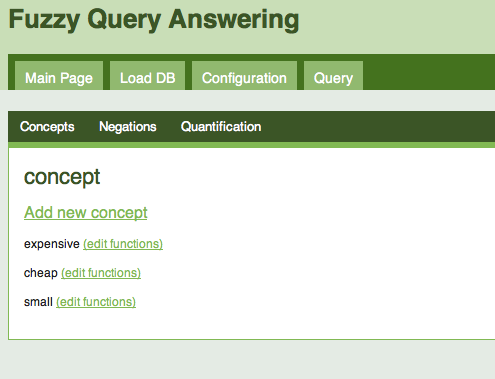
\includegraphics[scale=0.6]{Configuration.png}
\end{center}
\caption{Interface of Configuration Module}
\label{fig:CMI}
\end{figure}
As shown in figure \ref{fig:CMI}, the existing fuzzy concepts, negations and quantifications are shown by clicking subtitles ``Concepts", ``Negations" and ``Quantifications", respectively. In each page, users can click ``Add New concept", ``Add New negation" and ``Add New Quantification" to enter Adding pages.  Users can click hyperlink ``edit function" behind the fuzzy concept, negation or quantification you want to edit to enter the Editing page.
\newpage
\begin{figure}[h]
\begin{center}
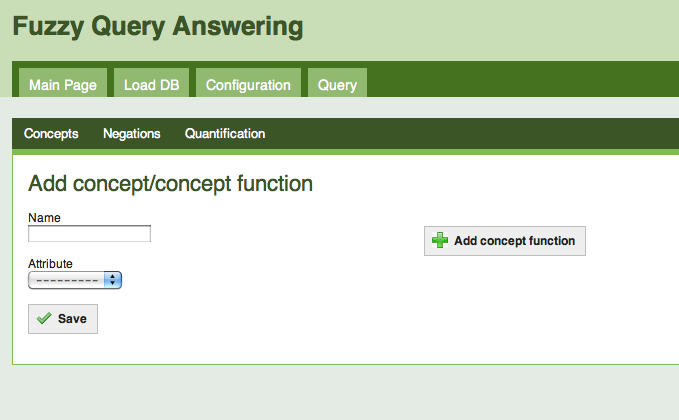
\includegraphics[scale=0.6]{AddingNewConcept.png}
\end{center}
\caption{Interface of adding new concept}
\label{fig:AddNewConceptInterface}
\end{figure}
As shown in figure \ref{fig:AddNewConceptInterface}, users can give the name of fuzzy concepts in ``Name" edit box, and choose an attribute from ``Attribute" selection box. For example, putting ``big" in ``Name" edit box and choosing ``size" from ``Attribute" selection box, in order to create a concept ``big" over attribute ``size". User can continue to add concept functions for this fuzzy concept by clicking ``Add concept function" in the case of adding functions for this fuzzy concept, then save both fuzzy concept and its functions. 
\newpage
\begin{figure}[h]
\begin{center}
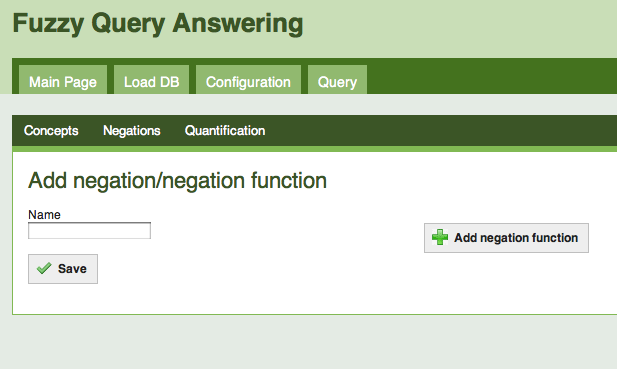
\includegraphics[scale=0.6]{AddingNewNegation.png}
\end{center}
\caption{Interface of adding new negation}
\label{fig:AddNewNegationInterface}
\end{figure}
As shown in figure \ref{fig:AddNewNegationInterface}, adding negation and adding quantification are the same, users only need to type the name of negation or quantification and click button ``Save". Before saving, users can also add functions of negation or quantification by clicking ``Add negation function" or ``Add quantification function".
 \newpage
\begin{figure}[h]
\begin{center}
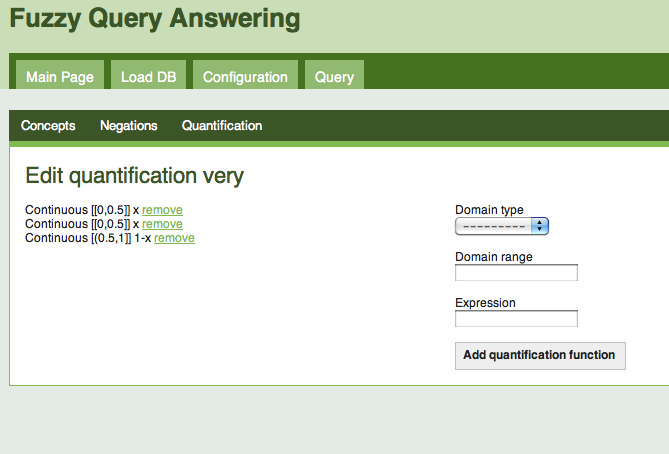
\includegraphics[scale=0.6]{EditingQuantification.png}
\end{center}
\caption{Interface of editing quantification}
\label{fig:EditQuantification}
\end{figure}
For editing functions, it is the same for fuzzy concepts, negations, and quantifications. As shown in figure \ref{fig:EditQuantification}, users can click hyperlink ``edit functions" behind the fuzzy concept, negation, quantification you want to edit. After entering the page of editing functions, users can remove the certain existing functions by clicking the hyperlink ``remove". In order to add more functions, users can choose the function type  from selection box ``Domain type", and type function domain in edit box ``Domain range", then write function expression in edit box ``Expression", the last step is to click button ``Add quantification function" in the case user edits quantification functions. The new function will be added to the list of functions on the left.



\newpage
\subsection{Query-Answering Module}
\label{sec:QAModule}
Query-Answering Module offers users to create simple fuzzy queries or complex fuzzy queries by choosing negations, quantifications and fuzzy concepts which are defined in Configuration Modules. 
% Theoretical definition of Fuzzy Query
% Explain the functionality of Query-Answering Module
% How to use Interface
\subsubsection{Fuzzy Query}
In RFuzzy Framework, we define the fuzzy query as a pair $<A,v>$, where $A \in TB_{\Pi,\Sigma,V}$ and $v$ is either a ``new'' variable that represents the initially unknown truth value of $A$ or it is a concrete value $v \in [0,1]$ that is asked to be the truth value of $A$. We extend this simple query into complex one.

\begin{defin} \textbf{(Complex fuzzy query).}
\label{def:ComplexFuzzyQuery}
\[Answer(\vec{t},v) \stackrel{c,F_c}{\longleftarrow} F(p_1(\vec{t_1},v_1),...,p_m(\vec{t_m},v_m))\]
where $p_i$s are predicates in RFuzzy program $P$, $Answer$ is a predicate which never appears in program $P$, $v_i$ and $v$ could be unknown truth value for their associated atoms or concrete value $v$ assigned to their atoms.

\end{defin}

By introducing quantifiers into RFuzzy framework, it could be used to enhance the expressivity of the query, which is defined as follow,

\begin{defin} \textbf{(Simple fuzzy query with negation and quantification). }
\label{def:SFQNegQuan}
\[< A,v >\]
where $A$ is an atom $q(x_1, \dots, x_n)$. $q$ is represented as a regular expression, 
\[q= (Negation|Quantification)^*Predicate\]
\end{defin}

\begin{defin} \textbf{(Complex fuzzy query with negation and quantification). }
\label{def:CFQNegQuan}
\[Answer(\vec{t},v) \stackrel{c,F_c}{\longleftarrow} F(q_1(\vec{t_1},v_1),...,q_m(\vec{t_m},v_m))\]
where $Answer$ is a predicate that never appears in program $P$, $q_i$ is represented as a regular expression, 
\[q_i = (Negation|Quantification)^*Predicate\]
\end{defin}

\begin{ex}
A set of negations is $N=\{not, seldom\}$, a set of quantifiers is $Q=\{very, extremely\}$, and a set of fuzzy concept is $C=\{beautiful, clear\}$. The simple query with negation and quantification can be represented as `` not very beautiful girls ?", ``seldom extremely clear statements ?" and so on. A Complex query with negation and quantification is generated by joining those simple query together with fuzzy rules. The simplest complex query could be `` not very beautiful and seldom extremely clear landscape ?", which is formalized in fuzzy logic as,
\begin{align*}
Answer(Landscape, V) {\longleftarrow} & \textbf{min} & not(very(beautiful(Landscape))),\\ 
&  & seldom(extremely(clear(Landscape))). \\
\end{align*}
\end{ex}

\subsubsection{How to use interface of Query-Answering Module}
\begin{figure}[htb]
\begin{center}
\leavevmode
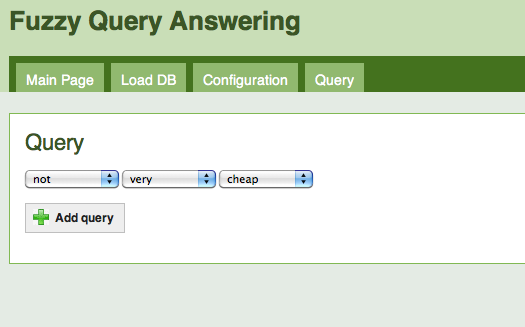
\includegraphics[scale=0.7]{Query.png}
\end{center}
\caption{Interface of Query-Answering Module}
\label{fig:QAMI}
\end{figure}
As shown in figure \ref{fig:QAMI}, users can choose negation, quantification, and fuzzy concept from  those three selection boxes. Users can add more queries by clicking button ``Add query", the previous query is listed on the right, and selection boxes are set to default empty ready for you to add more queries. By clicking button ``Query", the result will be generated and shown in a result page.

\end{document}